\documentclass[aspectratio=169]{beamer}
\usetheme{Madrid}
\usepackage{booktabs}
\usepackage{graphicx}
\usepackage{array}

\title{Branch Specialization Checkpoint}
\subtitle{Weakly Supervised Branch Routing}
\author{Branch Specialization Project}
\date{2026-05-22}

\begin{document}

\begin{frame}
  \titlepage
  \vspace{-0.5em}
  \begin{center}
    Checkpoint reason: weak routing supervision produced near-oracle learned modularity.
  \end{center}
\end{frame}

\begin{frame}{Question}
  Previous checkpoint:
  \begin{itemize}
    \item unconstrained learned routers solved the task;
    \item they did not recover role-specific branch modularity;
    \item oracle routing showed that modularity is possible in this setup.
  \end{itemize}

  \vspace{0.8em}
  This checkpoint asks:

  \begin{quote}
    Is a small scored-position routing signal sufficient for learned functional
    modularity to emerge?
  \end{quote}
\end{frame}

\begin{frame}{Setup}
  Same local-vs-induction competition task:
  \begin{itemize}
    \item local copy positions predict \texttt{x} from \texttt{[x, SEP, x]};
    \item induction positions predict the next token in a repeated random sequence;
    \item local weight 0.25, induction weight 1.0;
    \item five seeds per config, 1200 training steps.
  \end{itemize}

  \vspace{0.6em}
  New intervention:
  \begin{itemize}
    \item weak auxiliary routing loss, weight 0.05;
    \item local scored positions target branch 0;
    \item induction scored positions target branch 1;
    \item branch modularity is still measured by causal branch ablation.
  \end{itemize}
\end{frame}

\begin{frame}{Main Comparison}
  \begin{center}
  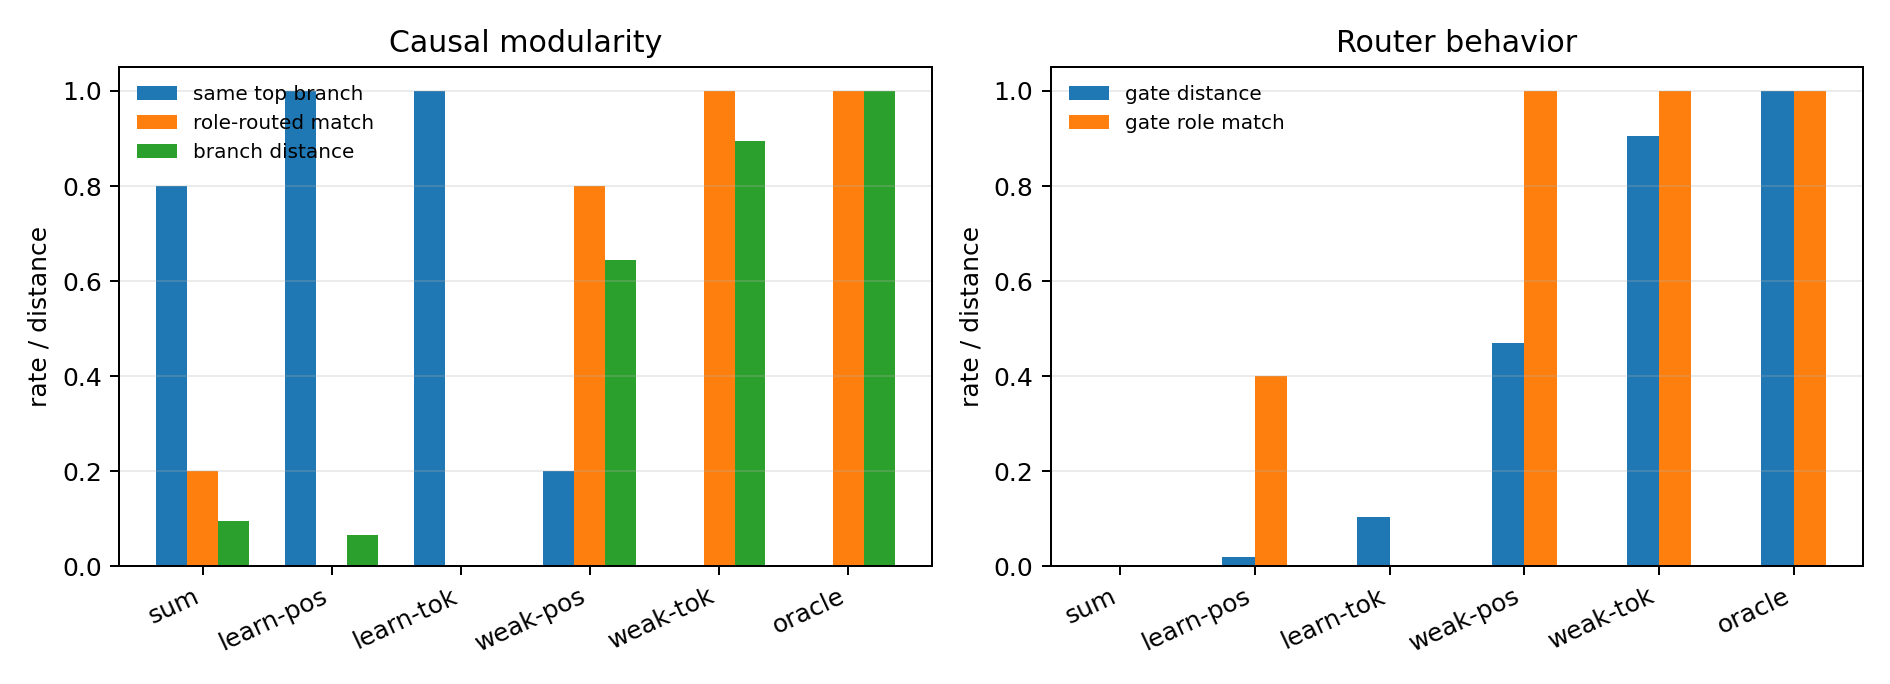
\includegraphics[width=0.9\linewidth]{figures/weak_router_comparison.png}
  \end{center}

  \vspace{-0.4em}
  \small
  Weak token routing moves from the entangled learned-router regime to near the
  oracle regime on both gate behavior and causal branch modularity.
\end{frame}

\begin{frame}{Modularity Table}
  \begin{center}
  \scriptsize
  \begin{tabular}{lrrrrr}
    \toprule
    Config & Local acc. & Ind. acc. & Same top & Routed match & Branch distance \\
    \midrule
    \texttt{branch\_sum} & 1.0000 & 0.9997 & 0.80 & 0.20 & 0.0951 \\
    \texttt{learned\_pos} & 0.9999 & 0.9987 & 1.00 & 0.00 & 0.0665 \\
    \texttt{learned\_tok} & 1.0000 & 0.9989 & 1.00 & 0.00 & 0.0006 \\
    \texttt{weak\_pos} & 0.9999 & 0.9988 & 0.20 & 0.80 & 0.6446 \\
    \texttt{weak\_tok} & 0.9998 & 0.9983 & 0.00 & 1.00 & 0.8957 \\
    \texttt{oracle} & 1.0000 & 0.9988 & 0.00 & 1.00 & 1.0000 \\
    \bottomrule
  \end{tabular}
  \end{center}

  \vspace{0.6em}
  Routed match means local depends most on branch 0 and induction depends most
  on branch 1 under ablation.
\end{frame}

\begin{frame}{Gate Behavior}
  \begin{center}
  \scriptsize
  \begin{tabular}{lrrrrr}
    \toprule
    Config & Gate match & Gate distance & Local entropy & Ind. entropy & Target NLL \\
    \midrule
    \texttt{weak\_pos} & 1.00 & 0.4700 & 0.4811 & 0.6422 & 0.3139 \\
    \texttt{weak\_tok} & 1.00 & 0.9049 & 0.0125 & 0.1944 & 0.0634 \\
    \bottomrule
  \end{tabular}
  \end{center}

  \vspace{0.8em}
  The token router learned much sharper gates. The position router followed the
  target direction, but remained softer and failed in one of five seeds.
\end{frame}

\begin{frame}{Branch Ablation}
  \begin{center}
  \scriptsize
  \begin{tabular}{lrrrr}
    \toprule
    Config & Local B0 & Local B1 & Induction B0 & Induction B1 \\
    \midrule
    \texttt{learned\_tok} & 2.2221 & 2.7767 & 2.3307 & 3.2506 \\
    \texttt{weak\_pos} & 0.9813 & 0.0406 & 0.5780 & 1.3542 \\
    \texttt{weak\_tok} & 5.6793 & 0.0000 & 0.5184 & 4.8444 \\
    \texttt{oracle} & 5.8198 & 0.0000 & 0.0000 & 6.1639 \\
    \bottomrule
  \end{tabular}
  \end{center}

  \vspace{0.7em}
  Weak token routing makes local branch 0 almost oracle-like. Induction mostly
  uses branch 1, but still has residual dependence on branch 0.
\end{frame}

\begin{frame}{Interpretation}
  \textbf{Supported in this toy setup:}
  \begin{itemize}
    \item Weak scored-position routing supervision is sufficient for learned
      branch-level functional modularity.
    \item Token-dependent routing is cleaner than position-only routing.
    \item Gate modularity and causal modularity now move together for the token router.
  \end{itemize}

  \vspace{0.6em}
  \textbf{Not shown:}
  \begin{quote}
    Spontaneous modularity without role labels. The auxiliary loss directly names
    the desired role split.
  \end{quote}
\end{frame}

\begin{frame}{Decision}
  Continue Phase 3 with two sharper tests:

  \begin{enumerate}
    \item sweep lower supervision weights to estimate the minimum signal needed;
    \item test unlabeled routing pressure, such as entropy or load-balancing
      regularization, and a more conflict-heavy task.
  \end{enumerate}

  \vspace{0.8em}
  Current working claim:
  \begin{quote}
    Learned functional modularity is possible here, but it needs routing pressure;
    gates without pressure did not find it on their own.
  \end{quote}
\end{frame}

\begin{frame}{Sources and Provenance}
  \scriptsize
  \begin{itemize}
    \item Report: \texttt{doc/phase3\_toy\_weak\_router.md}
    \item Model script: \texttt{scripts/toy\_branch\_isolation\_intervention.py}
    \item Weak-router output: \texttt{results/phase3\_toy\_weak\_router\_w005\_lw025/}
    \item Combined comparison: \texttt{results/phase3\_toy\_weak\_router\_w005\_combined/}
    \item Deck data snapshot: \texttt{presentations/2026-05-22-1300-weak-router/data/}
  \end{itemize}
\end{frame}

\end{document}
